\chapter{Theory and methods}
\label{chap:theory}
%\begin{quote}
% \textit{This chapter discusses the theory of energy transfer.}
%\end{quote}


In the publications included in this thesis, we have employed molecular dynamics (MD) simulations and Green's function (GF) calculations to model vibrational heat transfer in nanostructures. It is common to both of these methods that one needs to choose how to describe interatomic interactions and the coupling to external heat baths. Before describing MD and GF calculations in Secs. \ref{sec:md} and \ref{sec:gf}, we therefore briefly review the chosen interatomic potentials and the theory of Langevin heat baths below in Secs. \ref{sec:th_interatomicpotential} and \ref{sec:th_langevin}. When discussing the MD method, we also present the recently developed expression for the spectral heat current distribution.

For electromagnetic energy transfer, we have employed the same Langevin theory as in vibrational heat transfer to describe the microscopic dipolar thermal fluctuations. This theory is presented in Sec. \ref{sec:em_methods}

\section{Vibrational heat transfer}

\subsection{Theoretical background}
\label{sec:theory_vibtheory}
%As discussed in Chap. 1, propagating lattice vibrations carry heat in crystalline solids, and the quanta of such propagating vibrations are called phonons. The theoretical description is based essentially on the equations of motion for the atoms in the solid. Because fully quantum description does not easily allow for accounting for non-linear dynamics, which play an essential role in any system with non-negligible phonon-phonon interactions, the discussion below treats the atomic dynamics classically. 

%\begin{itemize}
% \item The goals of this work
%\end{itemize}
The theoretical description of lattice heat transfer is based on the dynamical equations of motion for the atoms constituting the lattice. The equations of motion are generally dictated by the Hamiltonian \cite{ziman}
\begin{equation}
 \ca{H} = \sum_{i=1}^N \frac{\bb{p}_i^2}{2m_i} + \ca{V}(\bb{r}_1,\dots,\bb{r}_N). \label{eq:th_hamiltonian}
\end{equation}
Here $\br_i$, $\bp_i$, and $m_i$ are the position, momentum and mass of atom $i$, respectively. The total number of atoms (which can also be infinite) is denoted by $N$. The first term of Eq. \eqref{eq:th_hamiltonian} is the total kinetic energy of the atoms and the second term $\ca{V}$ is the interatomic potential energy responsible for the interatomic interactions. The choice of the potential energy function $\ca{V}$ is crucial for an accurate description of the lattice dynamics and, consequently, of energy transfer. Models for $\ca{V}$ used in this work are explained in detail in Sec. \ref{sec:th_interatomicpotential}.

Applying Hamilton's equations of motion $\dot{\br}_i=\partial H/\partial \bp_i$ and $\dot{\bp}_i=-\partial \ca{H}/\partial \br_i$ \cite{fetter} gives Newton's law
\begin{equation}
 m_i \ddot{\br}_i = \bb{F}_i, \label{eq:th_eom}
\end{equation}
where the force acting on atom $i$ is
\begin{equation}
 \bb{F}_i = - \frac{\partial \ca{V}}{\partial \bb{r}_i}. \label{eq:th_force}
\end{equation}
For given initial conditions $\br_i(0)$ and $\dot{\br}_i(0)$, Eq. \eqref{eq:th_eom} determines the time evolution of atomic trajectories. To model energy transfer, the equations of motion are supplemented by terms accounting for coupling to external heat baths. In this work, we mostly employ Langevin heat baths that turn the equations of motion into stochastic equations and ensure that the long-term atomic trajectories correctly sample the non-equilibrium statistical ensemble. Langevin theory is presented in Sec. \ref{sec:th_langevin}.

Equation \eqref{eq:th_eom} generally describes the motions of atoms and molecules in solid, gas, and liquid systems. In solids, the atoms vibrate close to their equilibrium positions $\br_i^0$ and one can gain more insight into the lattice dynamics by only considering small displacements from the equilibrium. The positions $\br_i^0$ are defined by the condition of zero force:
\begin{equation}
 \left. \frac{\partial \ca{V}}{\partial \br_i} \right|_{\br_j=\br_j^0 \quad \forall j} = 0. \label{eq:th_zeroforce}
\end{equation}
Assuming that the atoms remain close to the equilibrium positions, one can expand the potential energy in Taylor series in terms of the displacements $\bu_i=\br_i-\br_i^0$:
\begin{equation}
 \ca{V} = \ca{V}_0 + \frac{1}{2} \sum_{i,j} \sum_{\alpha,\beta} u_i^{\alpha} K_{ij}^{\alpha \beta} u_j^{\beta}  + \ca{O}(u^3). \label{eq:th_V_taylor}
\end{equation}
Here the Cartesian coordinate directions $\alpha,\beta \in \{x,y,z\}$ have been written explicitly for clarity and the second-order term is proportional to the ''force constant''
\begin{equation}
 K_{ij}^{\alpha\beta} = \left. \frac{\partial^2 \ca{V}}{\partial u_i^{\alpha} \partial u_j^{\beta}} \right|_{\bu=\mathbf{0}}. \label{eq:th_K_def}
\end{equation}
The first-order derivative term in \eqref{eq:th_V_taylor} vanished based on Eq. \eqref{eq:th_zeroforce} and the last term is of third order in displacements.

In the case that the third-order term can be neglected, employing Eq. \eqref{eq:th_V_taylor} in the equation of motion \eqref{eq:th_eom} gives the system of linear equations
\begin{equation}
 m_i \ddot{u}_i^{\alpha} = - \sum_j \sum_{\beta} K_{ij}^{\alpha\beta} u_j^{\beta}.
\end{equation}
Following standard eigenmode theory \cite{fetter}, the eigenmodes of the system can be found by diagonalizing the matrix $D_{ij}^{\alpha\beta} = (m_i\omega^2 \delta_{ij}\delta
^{\alpha\beta}-K_{ij}^{\alpha\beta})$. In a periodically repeating crystal, the eigenmodes can be labeled by the wavevectors $\bb{q}$ belonging to the first Brillouin zone \cite{ziman} and the branch $p \in \{1,\dots,3N_{\textrm{cell}}\}$, where $N_{\textrm{cell}}$ is the number of atoms in the unit cell. The eigenmodes are called phonon modes, while phonons are the discrete quanta of eigenmode occupation. The eigenfrequencies $\omega(\bb{q},p)$ form the phonon bandstructure, specifying the relation between the wavevectors and frequencies supporting propagating phonon modes. As an example, Fig. \ref{fig:th_nika} shows the phonon bandstructure of graphene, a single monolayer of graphite.

\begin{figure}
\begin{center}
 \includegraphics[width=8.6cm]{pics/nika09_fig3.pdf}
 \caption{Phonon bandstructure of graphene, calculated using the valence force field method \cite{nika09}. The two-dimensional bandstructure is plotted along one-dimensional lines between special points in graphene reciprocal lattice, denoted by $\Gamma$, $M$ and $K$. Because graphene has two atoms per unit cell, there are altogether six phonon branches. The three branches that have vanishing frequencies at the $\Gamma$ point are called longitudinal acoustic (LA), transverse acoustic (TA) and out-of-plane acoustic (ZA). The optical modes LO, TO and ZO are labeled similarly. Reprinted with permission from Ref. \cite{nika09}.}
\label{fig:th_nika}
\end{center}
\end{figure} 

When the anharmonic part in Eq. \eqref{eq:th_V_taylor} is neglected, the phonon eigenmodes are exact eigenmodes of the system and cannot dissipate their energy, giving rise to infinite thermal conductivity \cite{ziman}. The anharmonic terms give rise to phonon-phonon scattering \cite{ziman}, which is the primary phonon decay mechanism in crystalline solids at high temperatures. In Publications \cp{fpu}, \cp{fpu2}, \cp{spectral}, \cp{cnt}, and \cp{twinning}, we have employed classical molecular dynamics simulations fully accounting for anharmonic scattering. In \citepub{gf}, anharmonic effects are mimicked by the self-consistent heat bath model \cite{bolsterli70}, allowing for the inclusion of quantum statistics as well. These methods are explained in more detail below in Chap. XXX.

\subsection{Models for interatomic potential energy}
\label{sec:th_interatomicpotential}

%Typically, the analytical form of the interatomic potential is inferred from quantum-mechanical calculation and the free parameters are fitted to reproduce experimentally known quantities such as the lattice constant, bulk modulus, atomization energy, and so on. For this reason, the interatomic potentials are often called semi-empirical. In chemistry, the term force field is used instead of interatomic potential.

As mentioned in Sec. \ref{sec:intro_vibtheory}, a crucial physical aspect of correctly describing the lattice dynamics and, therefore, vibrational energy transfer is the choice of interatomic potential energy function $\ca{V}$. In general, the interatomic potential consists of pair potential terms and many-body terms. 
%, which we assume to only consist of the three-body terms $V^{(3)}(\bb{r}_i,\bb{r}_j,\bb{r}_k)$:
%\begin{equation}
% U(\bb{x}) = \frac{1}{2}  \sum_{ i,j } V^{(2)}(|\bb{r}_{i}-\bb{r}_j|) + \frac{1}{6} \sum_{i,j,k} V^{(3)}(\bb{r}_i,\bb{r}_j,\bb{r}_k)
%\end{equation}
A very simple example of a pure pair-potential is the Fermi-Pasta-Ulam (FPU) potential used by Fermi, Pasta, and Ulam to investigate the minimal necessary conditions for thermalization in one-dimensional system. In the FPU model, atoms with displacement $u_i$ from the equilibrium position are assumed to be connected to their nearest neighbors by anharmonic springs with the pair-wise energy of the form
\begin{equation}
  V_{ij}^{\textrm{FPU}} = \frac{1}{2} k (u_i-u_j)^2 + \frac{\alpha}{3} (u_i-u_j)^3+ \frac{\beta}{4} (u_i-u_j)^4, \label{eq:th_fpu}
\end{equation}
which is referred to as the FPU potential. The FPU potential can be considered to arise from the Taylor expansion of a more realistic potential (such as LJ). The models for $\beta=0$ and $\alpha=0$ are known as $\alpha$-FPU and $\beta$-FPU, respectively, and both have been employed extensively in investigating thermalization and thermal conduction in low-dimensional systems \cite{}. In Publications \cp{fpu} and \cp{fpu2}, the $\beta$-FPU potential was used to model the anharmonic interactions in a square lattice. In Publication \cp{gf}, the anharmonic interactions were mimicked by the coupling to self-consistent heat baths (see Sec. \ref{sec:gf}), and only the harmonic term of Eq. \eqref{eq:th_fpu} was included ($\alpha=\beta=0$).

Another very common pair-potential is the Lennard-Jones (LJ) potential \cite{allentildesley}
\begin{equation}
 V_{ij}^{\textrm{LJ}}(r_{ij}) = 4\varepsilon \left[\left( \frac{\sigma}{r_{ij}}\right)^{12}-\left( \frac{\sigma}{r_{ij}}\right)^6  \right],
\end{equation}
where $\varepsilon$ is the interaction energy, $\sigma$ determines the equilibrium distance $r_0$ of atoms ($r_0=2^{1/6}\sigma$ for two particles), and $r_{ij}$ is the interparticle distance. The repulsive term $(\sigma/r_{ij})^{12}$ models the strong atomic repulsion at short distances, arising from the overlapping of electron clouds. The attractive term $-(\sigma/r_{ij})^{6}$ accounts for the weak van der Waals attraction at large distances, arising from the interaction of the fluctuating dipole moments due to, e.g., electron polarization. The LJ potential accurately describes interatomic interactions between noble gas atoms such as argon and, thanks to its simple form, it is also often used to investigate the qualitative features of heat transfer in solids \cite{}. The LJ potential was used in Publication \cp{spectral} to model the interatomic interactions in investigating the spectral conductance between mass-mismatched solids arranged in a face-centered cubic lattice. %Because the LJ interaction does not account for the local environment, however, the LJ potential cannot describe, e.g., covalent bonding. %It is used a constituent in more complicated potentials to describe the van der Waals attractions. Due to its simple form, it is also often used 


Pure pair-potentials such as the Lennard-Jones potential cannot describe, e.g., covalent bonding, where the strength of local bonding is strongly influenced by the environment. Therefore, a more sophisticated potential is needed to model, for example, carbon materials. A typical example of a many-body potential is the Tersoff potential \cite{tersoff88b}
\begin{equation}
 V_{ij}(r_{ij}) = f_C(r_{ij}) \left[A e^{-\lambda_1 r_{ij}} - B b_{ij} e^{-\lambda_2 r_{ij}}) \right],
\end{equation}
where the taper function 
\begin{equation}
 f_C ( r) = \left\{ \begin{array}{ll}
                     1 & \textrm{for } r<R-D,\\
		     \frac{1}{2}-\frac{1}{2}\sin\left(\frac{\pi}{2}\frac{r-R}{D} \right) & \textrm{for } R-D < r < R+D, \\
		     0 & \textrm{for } r>R+D
                    \end{array}
 \right.
\end{equation}
gradually turns off the pair-wise interaction between $r_{ij}=R-D$ and $r_{ij}=R+D$. The strength of interatomic attraction is controlled by the coefficient
\begin{equation}
 b_{ij} = \left( 1+\beta^n \zeta_{ij}^n \right)^{-1/(2n)},
\end{equation}
where the dependence on the local environment appears in the definition 
\begin{equation}
 \zeta_{ij} = \sum_{k\neq i,j} f_C(r_{ik}) g(\Theta_{ijk}) \exp\left[\lambda_3^3(r_{ij}-r_{ik})^3 \right] .
\end{equation}
Here $\Theta_{ijk}$ is the angle between bonds $ij$ and $ik$. The angle function is defined as 
\begin{equation}
 g(\Theta) = 1 + \frac{c^2}{d^2} - \frac{c^2}{d^2 + (\cos \Theta-\cos \Theta_0)^2}
\end{equation}
The parameters $R$, $D$, $A$, $\lambda_1$, $B$, $\lambda_2$, $\beta$, $n$, $\lambda_3$, $c$, $d$, and $\Theta_0$ depend on the material under study. The Tersoff parameters for carbon systems were originally fit to the experimentally known cohesive energies of various carbon systems and the lattice constant and bulk modulus of diamond \cite{tersoff88a}. Recently, Lindsay and Broido \cite{lindsay10} suggested an improved set of parameters found by giving more weight to matching the experimentally measured phonon dispersion for graphite. This optimized Tersoff potential was used in Publication \cp{cnt} for carbon nanotubes. In \citepub{twinning}, many-body Stillinger-Weber potential \cite{stillinger85} was used to model interactions between Si atoms constituting Si nanowire. 


\subsection{Langevin theory} 
\label{sec:th_langevin}
The equations of motion \eqref{eq:th_eom} only describe the interactions between the constituents of the system under study. To enable steady-state energy transfer, some of the degrees of freedom must be coupled to external heat baths acting as heat sources and sinks. Because Langevin heat baths are employed in all but one publication included in this thesis, we briefly review the Langevin theory.

In Langevin theory, the particle coupled to the bath is imagined to interact with a collection of harmonic oscillators at a prescribed temperature. The bath degrees of freedom are ''integrated out'' so that their interaction with the system under study is described effectively by the Langevin forces \cite{weiss}. The general Langevin equation obtained through such a procedure reads \cite{dhar06}
\begin{equation}
 m\ddot{\bu}_i(t) =  \bb{F}_i(t) - \int_{0}^{\infty}dt' \Sigma_i(t') \bb{u}_i(t-t') + \xi_i(t), \label{eq:th_eom_langevin}
\end{equation}
where, for the simplicity of discussion, we assume that the baths are spatially uncorrelated so that the bath self-energy $\Sigma_i$ is spatially local. The self-energy describes the dynamical interactions and damping induced by the coupling to the heat bath oscillators. The force $\bb{F}_i$ is due to interactions with particles not in the reservoir and the auto-correlation function of the random force $\xi_i$ is related to the damping self-energy $\Sigma_i(t)$ and bath temperature $T_i$ through the fluctuation-dissipation theorem (FDT) \cite{dhar06}
\begin{equation}
 \langle \xi_i(t)\xi_i(t') ^T\rangle = \int_{-\infty}^{\infty} \frac{d\omega}{2\pi} e^{-i\omega(t-t')} \hbar \Gamma_i(\omega) \left[f_B(\omega,T_i)+\frac{1}{2}\right] \bb{I}_{3\times3}. \label{eq:th_xixit}
\end{equation}
Here $\Gamma_i(\omega)=-2\textrm{Im}[\Sigma_i(\omega)]$ is called the bath coupling function \cite{dhar06}. The quantum statistics appear through the Bose-Einstein occupation function $f_B(\omega,T)=\left\{\exp[\hbar\omega/(k_BT)]-1 \right\}^{-1}$. By Fourier transforming with respect to $t$ and $t'$ separately, Eq. \eqref{eq:th_xixit} can be written in the form useful for calculations:
\begin{equation}
  \langle\tilde  \xi_i(\omega)\tilde \xi_i(\omega')^T \rangle = 2\pi\hbar\delta(\omega+\omega') \Gamma_i(\omega) \left[f_B(\omega,T_i)+\frac{1}{2} \right] \bb{I}_{3\times3}. \label{eq:th_xixiom}
\end{equation}

To simulate Langevin dynamics in a MD simulation, it is useful to write the integral term appearing in the Langevin equation in terms of the velocity $\dot{u}(t)$. To achieve this, one can integrate in Eq. \eqref{eq:th_eom_langevin} partially to get
\begin{equation}
 m\ddot{\bu}_i(t) =  \bb{F}_i(t) - \int_{0}^{\infty}dt' M(t')\dot{\bb{u}}_i(t-t') + \xi_i(t). \label{eq:th_langevin_Mt}
\end{equation}
The boundary terms appearing in the partial integration are assumed to vanish because we (i) define the integral function $M(t)=-\int_t^{\infty} dt' \Sigma(t')$ of $\Sigma(t)$ for positive $t$ so that $M(t\to \infty)=0$ and (ii) the term proportional to $M(0)u(t)$ can be absorbed to the external force $F[u(t)]$ or eliminated by re-defining the displacements \cite{weiss}. The classical Langevin equation is obtained by choosing a very rapidly decaying $M(t)$ and taking the limit of vanishing decay time, allowing for arriving at the classic Langevin equation \cite{zwanzig}
\begin{equation}
 m\ddot{\bu}_i(t) =  \bb{F}_i(t) - m\gamma \dot{\bu}_i(t) + \xi_i(t). \label{eq:th_ohmic}
\end{equation}
This form of damping, proportional to the instantaneous velocity $\dot{\bu}(t)$ and the friction constant $\gamma$, is called Ohmic damping due to its analogue with a resistor in an electrical circuit \cite{weiss}. This form can be shown to give rise to a frequency-independent phonon relaxation time $\tau=1/\gamma$ \cite{li09jap}. The corresponding FDT \eqref{eq:th_xixiom} for the force variance is, for Ohmic damping,
\begin{equation}
 \langle \tilde \xi_i(\omega) \tilde \xi_i(\omega')^T \rangle = 4\pi \delta(\omega+\omega') \hbar \omega \gamma \left[f_B(\omega,T_i)+ \frac{1}{2} \right] \bb{I}_{3\times 3}. \label{eq:th_xixiom_ohmic_qm}
\end{equation}
In the classical high-temperature limit relevant for classical molecular dynamics, one gets the classical FDT \cite{zwanzig}
\begin{equation}
 \langle \xi_i(t) \xi_i(t')^T\rangle=2\gamma k_B T_i \delta(t-t') \bb{I}_{3\times 3}. \label{eq:th_corr_ohmic} 
\end{equation}

In this thesis, we employ the Ohmic damping of Eq. \eqref{eq:th_ohmic} due to its simplicity. In Publications \cp{fpu}, \cp{fpu2}, \cp{spectral}, and \cp{cnt}, Ohmic Langevin heat baths are used as hot and cold heat baths in the molecular dynamics simulation. In accordance with the classical dynamics, the classical FDT \eqref{eq:th_corr_ohmic} is employed for force variance. \citepub{twinning} employs the classical Nose-Hoover heat baths \cite{hoover85} instead of Langevin heat baths. In Publication \cp{gf}, Langevin heat baths act not only as external thermal reservoirs but also as pathways for phonon creation and annihilation inside the system under study. In Publication \cp{dipole}, Langevin baths are used to model thermal fluctuations and dissipation of dipole moments. Because the equations of motion are linear in the two latter cases, we can also account for quantum statistics by using the quantum fluctuation-dissipation theorem \eqref{eq:th_xixiom_ohmic_qm}.

\subsection{Molecular dynamics}
\label{sec:md}

Molecular dynamics simulations are a powerful tool for modeling the vibrational energy transfer in atomic scale systems. In MD, the classical Newton's equations of motion \eqref{eq:th_eom} [or more generally the Langevin equation \eqref{eq:th_ohmic} for atoms coupled to heat baths] are integrated numerically. The forces $\bb{F}_i$ are calculated from an analytical expression obtained from the interatomic potential function $\ca{V}$ as $\bb{F}=-\partial \ca{V}/\partial \bb{r}_i$ and therefore include all orders of anharmonic terms. By simulating the steady-state non-equilibrium for sufficiently long times, one can extract values of macroscopic observables such as the heat current accurately by time-averaging. Based on the ergodicity principle, the time averages are expected to equal the statistical average over the corresponding ensemble. In the following, we briefly go through the most important aspects related to a MD simulation.

% One key aspect of the method is the assumption of ergodicity: statistical ensemble average can be calculated from a time average, meaning that  %In a microcanonical simulation, for example, the system should sample all the states that lie on the constant-energy manifold determined by the initial conditions. 

In MD, the equations of motion are integrated numerically using a finite-difference method. The pool of the finite-difference methods includes, e.g., Euler methods, Verlet methods, Runge-Kutta methods, the leap-frog method and predictor-corrector methods \cite{allentildesley}. In all the simulations of this work, the velocity Verlet algorithm was employed to integrate the equations of motion. While velocity Verlet exhibits moderate short-term energy drift, it is very simple to implement, efficient and it possesses very small long-term energy drift due to its being both time-reversible and symplectic \cite{frenkelsmit}. The velocity Verlet update equations for the positions $\bb{r}_i$ and velocities $\bb{v}_i=\dot{\bb{r}}_i$ are \cite{allentildesley}
\begin{alignat}{2}
  \bb{r}_i(t+\Delta t) &= \bb{r}_i(t) + \bb{v}_i(t)\Delta t+  \frac{1}{2}\bb{a}_i(t) \Delta t^2 + \mathrm{O}(\Delta t^4) \\
  \bb{v}_i(t+\Delta t) &= \bb{v}_i(t) + \frac{ \bb{a}_i(t)+\bb{a}_i(t+\Delta t)}{2} \Delta t+ \mathrm{O}(\Delta t^2) ,
\end{alignat}
where $\Delta t$ is the time step and $\bb{a}_i(t)=\bb{F}_i(t)/m_i$ is the acceleration.

To outline the typical steps involved in a non-equilibrium simulation, consider the example setup of Fig. \ref{fig:intro_systems}(b) used to investigate the anharmonic effects in interfacial heat transfer. First the whole structure is equilibrated by running a zero-pressure simulation at prescribed temperature using a combination of a Nose-Hoover barostat and thermostat, allowing the structure to conform to zero-stress state. Typical equilibration period consists of a few hundreds of thousands of time steps. After the initial equilibration, the size of the simulation box is fixed, as are atoms located at the left- and right-most unit cells in the system. This prevents atomic sublimation at the free surfaces. Particles in the ''hot'' and ''cold'' regions, illustrated by the red and cyan coloured atoms in Fig. \ref{fig:intro_systems}(b), are coupled to heat baths at temperatures $T_{\textrm{hot}}$ and $T_{\textrm{cold}}$. The system is then allowed to reach non-equilibrium steady state by running MD until the temperature profile and the heat current flowing through the system fluctuate around constant values. After this initial period, simulation is continued typically for millions of time steps, and the values of the observables of interest are collected from the run. The statistical error in the collected observables can be estimated by using standard methods described, e.g., in \citepub{fpu}.


%\textbf{SIMULATION FLOW}

\subsubsection{Lattice heat current}
\label{sec:spectral}
The main observable of interest in heat transfer simulations is the heat current flowing through system, which can be expressed as a sum of interatomic heat currents flowing across a specified cross-section of the simulation domain. The expression for the interatomic heat current can be determined by calculating the temporal rate of change in the local energy consisting of kinetic and potential energy contributions \cite{hardy63,lepri03}. For the average heat current flowing from atom $j$ to atom $i$ one thereby gets (see \citepub{fpu} for derivation) 
\begin{equation}
 Q_{j\to i} = \left\langle \frac{1}{2} \bb{F}_{ij} \cdot \left( \bb{v}_i+\bb{v}_j \right) \right\rangle, \label{eq:th_Qji}
\end{equation}
where the force acting on atom $i$ due to the interaction with atom $j$ is obtained from the pairwise potential energy $V_{ij}$ as
\begin{equation}
 \bb{F}_{ij} = - \frac{\partial V_{ij}}{\partial \bb{r}_i}.
\end{equation}
The angular brackets in Eq. \eqref{eq:th_Qji} denote non-equilibrium ensemble average, which can be calculated by time-averaging in MD simulations. 

Equation \eqref{eq:th_Qji} cannot directly indicate, which vibrational frequencies are actually responsible for the energy transfer. Such an analysis was enabled in \citepub{spectral}, where an expression for the spectral decomposition $q_{j\to i}(\omega)$ of heat current was derived. The decomposition is defined implicitly through the formula
\begin{equation}
 Q_{j\to i} = \int_0^{\infty} \frac{d\omega}{2\pi} q_{j\to i}(\omega)
\end{equation}
and was shown to be given by the expression
\begin{equation}
 q_{j \to i}(\omega) = 2\textrm{Re} [\tilde K_{ij}(\omega)],
\end{equation}
where $\tilde K_{ij}(\omega)=\int_{-\infty}^{\infty} dt e^{i\omega t}K_{ij}(t)$ is the Fourier transform of the time-domain correlation function
\begin{equation}
 K_{ij}(t_1-t_2) = \frac{1}{2} \left\langle \bb{F}_{ij}(t_1) \cdot \left[ \bb{v}_i(t_2)+\bb{v}_j(t_2)\right] \right\rangle \label{eq:th_Kijt1t2}
\end{equation}
The force-velocity correlation function depends explicitly only on the time-difference $t_1-t_2$ due to the assumed steady-state. 

The correlation function can be calculated by analyzing the force and velocity trajectories obtained from non-equilibrium molecular dynamics simulation. In practice, it is useful expand the interatomic force $\bb{F}_{ij}$ in terms of small displacements from equilibrium positions, allowing for simplifying the post-processing and detailing the relative contributions of linear and non-linear energy transfer mechanisms. The contributions of non-linear terms to the interfacial thermal conductance were analyzed in \citepub{spectral}. In \citepub{cnt}, only the dominant linear term was included in investigating the phonon transmission in carbon nanotubes.


\section{Green's function methods}



\subsection{Self-consistent heat bath model}
\label{sec:gf}

\begin{figure}
\begin{center}
 %\includegraphics[width=8.6cm]{../scbaths_paper_re_resubmission/pic1.ps}
 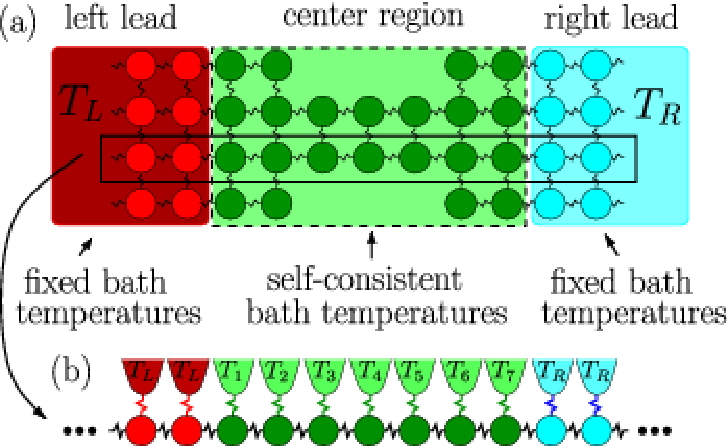
\includegraphics[width=8.6cm]{pics/pic_scbaths.pdf}
 \caption{(a) A schematic illustration of the system under study. The structure is divided into the left lead, the center region and the right lead. All atoms are coupled to spatially uncorrelated quantum Langevin heat baths, which are shown explicitly for one cross-section in (b). In the left and right lead, the temperatures of the local heat baths have prescribed values $T_L$ and $T_R$, respectively. In the center region, on the other hand, temperature varies between $T_L$ and $T_R$ and the bath temperatures are determined self-consistently using the requirement that the average thermal current to each bath vanishes. The leads can contain an infinite number of atoms, but the center region is finite. Two-dimensional square lattice with nearest neighbor interactions is shown for illustrative purposes, but the basic principle can be applied to any geometry.}
\label{fig:sud1}
\end{center}
\end{figure}

Quantum effects cannot be rigorously accounted for using molecular dynamics simulations. Therefore, one must find alternative methods to solve the equations of motion. The solution is, however, practically impossible due to the non-linear terms arising from the anharmonicity in the interatomic potential. The usual approach in traditional Landauer-B\"uttiker calculations \cite{zhang07} is to neglect the anharmonic terms, but then the model can only describe purely ballistic phonon transport. 

To account both for quantum statistical effects and non-ballistic transport, one can mimic the anharmonic terms responsible for phonon decay by an effective frictional term in the equation of motion. To be consistent with the fluctuation-dissipation theorem, the dissipative term must, however, be accompanied by a stochastic force term. The atoms are then effectively coupled to Langevin heat baths. The requirement of local current conservation leads to the requirement of solving the heat bath temperature self-consistently, leading to the self-consistent heat bath model described below. The self-consistent heat bath model was first proposed by Bolsterli, Rich, and Visscher to describe diffusive heat transfer in one-dimensional systems \cite{bolsterli70} and has since been used in multiple works investigating, e.g., the ballistic-diffusive transition in low-dimensional systems \cite{bonetto04,dhar06,roy08} and the necessary conditions for thermal rectification \cite{pereira08,segal09,bandyopadhyay11}.

The system under study is schematically illustrated in Fig. \ref{fig:sud1}. The setup resembles the classical Landauer-B\"uttiker setup \cite{datta}, consisting of the left lead region, center region and right lead region. Contrary to the Landauer-B\"uttiker setup, however, all atoms are coupled to ohmic Langevin heat baths mimicking scattering events such as phonon-phonon scattering driving the system towards local thermal equilibrium. In the leads, the bath temperatures are set to prescribed values $T_L$ and $T_R$. The atoms in the center region are coupled to local heat baths whose temperatures are determined self-consistently from the requirement of local current conservation. The presence of heat baths both in the leads and center region ensures perfect acoustic matching at the fictional interfaces separating the regions. %The coupling to the Langevin heat baths effectively .

To write down the equation of motion for the atoms, we observe that the time evolution consists of (1) the deterministic part, specified by the system Hamiltonian $\ca{H}$ and the Heisenberg equations of motion, and (2) the stochastic part due to the interaction with the heat baths.  Part (1) is specified by writing down the harmonic Hamiltonian for the system:
\begin{equation}
 \ca{H} = \frac{1}{2}  \sum_I \left[ \frac{\bb{p}_I^2}{m}+\bb{u}_I^T\bb{K}_I \bb{u}_I \right] + \sum_I \sum_{J\neq I} \bb{u}_I^T \bb{V}_{IJ} \bb{u}_J.
\end{equation}
The index $I\in\{C,L,R\}$ labels the region: $C$ stands for center region, and $L$ and $R$ for the left and right leads, respectively. For each index $I$, the atomic displacement vector $u_i^{\alpha}=r_i^{\alpha}-r_i^{\alpha 0}$ is defined as the displacement of position $r_i^{\alpha}$ from the equilibrium position $r^{\alpha 0}_i$, where $\alpha\in\{x,y,z\}$. The atomic momenta are in vectors $\bb{p}_I$. We assume the masses $m$ of all atoms to be equal. The spring constant matrix $\bb{K}_I$ and the inter-region coupling matrices $\bb{V}_{IJ}$ are the blocks of the full spring constant matrix $\bb{K}$ [Eq. \eqref{eq:th_K_def}]:
\begin{equation}
 \bb{K} = \left(\begin{matrix}
                 \bb{K}_L & \bb{V}_{LC} & 0 \\
		\bb{V}_{CL} & \bb{K}_C & \bb{V}_{CR} \\
		0 & \bb{V}_{RC} & \bb{K}_R.
                \end{matrix}
 \right)
\end{equation}
 
The Heisenberg equations of motion, which coincide with the classical equations of motion $m\ddot{\bb{u}}_I=-\partial \ca{H}/\partial \bb{u}_I$ due to the linearity of the system, can be determined from the Hamiltonian. Accompanied with the non-Hamiltonian time-evolution arising from the Ohmic interaction with the heat bath [see Eq. \eqref{eq:th_ohmic}], the equations of motion are then
\begin{equation}
  m\ddot{\bb{u}}_I = - \bb{K}_I \bb{u}_I - \sum_{J\neq I} \bb{V}_{IJ} \bb{u}_J - m \gamma \dot{\bb{u}}_I + \xi_I. \label{eq:gfm_eom_I}
\end{equation}

Our goal is to derive an explicit solution for the atomic dynamics $\bb{u}_C$, from which one can calculate the time-averages of heat currents both to the leads and to the local baths. The expression for $\bb{u}_C$ can be determined by (1) eliminating the time derivatives by temporal Fourier transform and (2) solving the equation of motion for $\bb{u}_L$ and $\bb{u}_R$ and substituting to the equation of $\bb{u}_C$. As shown in detail in \citepub{dipole}, one gets
\begin{equation}
 \hat{\bb{u}}_C(\omega) = - \bb{G}(\omega) \left[ \hat\xi_C(\omega) + \sum_{I=L,R} \hat{\eta}_I(\omega) \right]. \label{eq:gfm_uc_sol}
\end{equation}
Here the Green's function for the center region is defined as the matrix inverse
\begin{equation}
 \bb{G}(\omega) = \left[m\omega^2 - \bb{K}_C(\omega) +im\gamma(\omega) - \sum_{I=L,R} \Sigma_I(\omega)  \right]^{-1}.
\end{equation}
The coupling to the leads appears only through the lead self-energies
\begin{equation}
 \Sigma_I(\omega) = \bb{V}_{CI} \bb{g}_I(\omega) \bb{V}_{IC} \label{eq:th_sigmaI}
\end{equation}
responsible for phonon ''leak'' to the leads and the lead-coupled Langevin noise terms
\begin{equation}
 \hat\eta_I(\omega) = \bb{V}_{CI}\bb{g}_I(\omega) \hat{\xi}_I(\omega). \label{eq:th_etaI}
\end{equation}
representing the stochastic arrival of phonons from the leads to the center region. The decoupled Green's function of the leads appearing in Eqs. \eqref{eq:th_sigmaI} and \eqref{eq:th_etaI} are
\begin{equation}
 \bb{g}_I(\omega) = \left[m\omega^2+im\gamma\omega - \bb{K}_I \right]^{-1}.
\end{equation}
As shown in \citepub{gf}, the lead noise terms $\hat\eta_I(\omega)$ satisfy the fluctuation-dissipation relation analogous to Eq. \eqref{eq:th_xixiom}:
\begin{equation}
 \langle \hat\eta_I(\omega) \hat\eta_I(\omega')^T \rangle=2\pi\delta(\omega+\omega') \Gamma^I(\omega) \left[f_B(\omega,T_I)+1 \right] \label{eq:th_etaIetaI}
\end{equation}
where $\Gamma^I(\omega)=-2\textrm{Im}[\Sigma_I(\omega)]$.

Having the solution \eqref{eq:gfm_uc_sol} and the fluctuation-dissipation relations for the local heat baths [Eq. \eqref{eq:th_xixiom_ohmic_qm}] and leads [\eqref{eq:th_etaIetaI}] available, one can calculate the heat currents flowing to the local heat baths and to the leads. As shown in Publication \cp{gf}, the heat current to the local heat baths (bath index $I\in \{1,\dots,N_C\}$, $N_C$ being the number of atoms in the center region) or to the leads ($I \in \{L,R\}$) can be written in the compact form
\begin{equation}
 \langle Q_I \rangle =  \int_0^{\infty} \frac{d\omega}{2\pi} \hbar \omega \sum_{J} \ca{T}_{IJ}(\omega)[f_B(\omega,T_J)-f_B(\omega,T_I)], \label{eq:gfm_qi}
\end{equation}
where the transmission function from lead $J$ to lead $I$ is the matrix trace 
\begin{equation}
 \ca{T}_{IJ}(\omega) = \textrm{Tr}[\Gamma^I(\omega) \bb{G}(\omega) \Gamma^J(\omega) \bG(\omega)^{\dagger}]. \label{eq:gfm_caroli}
\end{equation}
The coupling functions $\Gamma^I(\omega)$ are defined as $\Gamma^i(\omega)=2m\gamma\omega \bb{I}_{3\times3}$ for the local heat baths.

Equation \eqref{eq:gfm_qi} is the multiprobe Landauer-B\"uttiker formula \cite{buttiker92} for energy transfer between heat baths. Equation \eqref{eq:gfm_caroli} was first derived for electron energy transfer by Caroli \textit{et al.} \cite{caroli71} and later derived for phonon transfer from the mode picture \cite{mingo06} and Keldysh formalism \cite{yamamoto06}. In Publication \cp{gf}, we derived the formula using local Langevin heat baths and thereby also included dissipative effects in the leads.

As mentioned above, the bath temperatures in the center region must be determined self-consistently from the requirement of vanishing energy current (Eq. \eqref{eq:gfm_qi}] to the baths. Because the bath temperatures $T_i$ appear in the Bose-Einstein function in the expression for the current, one must solve a non-linear system of equations. The solution to the system of equations can be determined exactly by using, e.g., the Newton-Raphson method \cite{bandyopadhyay11} or approximately by linearizing the equations in terms of temperatures \cite{segal09}. In \citepub{gf}, we compared the exact and linearized solutions and also suggested an alternative method for solving the equations, based on considering the transient time evolution of bath temperatures and integrating the time evolution equations until steady-state is achieved. 

%\textbf{Solution of self-consistent equations}

\section{Methods for electromagnetic energy transfer}

\subsection{Theoretical background}

\label{sec:theory_emtheory}

\subsubsection{Field due to an oscillating dipole}

The theoretical description of electromagnetic energy transfer between oscillating dipoles is based on Maxwell equations \cite{novotny}. In the non-magnetic materials with no free charges that are considered in this work, the electromagnetic fields arise from the fluctuating electric polarization fields inside the bodies, and the Maxwell equations for the electric field $\bE(\br,t)$ and magnetic field $\bb{H}(\br,t)$ read \cite{novotny}
\begin{subequations}
\begin{align}
  \nabla \times \bE(\br,t) &= - \mu_0 \frac{\partial \bb{H}(\br,t)}{\partial t}, \label{eq:th_maxwell1} \\
  \nabla \times \bb{H}(\br,t) &= \varepsilon_0 \frac{\partial \bb{E}(\br,t)}{\partial t} + \frac{\partial \bb{P}(\br,t)}{\partial t}, \label{eq:th_maxwell2} \\
   \nabla \cdot \bb{H}(\br,t) &= 0, \\
   \nabla \cdot \bb{E}(\br,t) &= 0.
\end{align}
\end{subequations}
Equation \eqref{eq:th_maxwell2} shows that a temporal change in the polarization density $\bb{P}(\br,t)$ gives rise to a magnetic field, which in turn induces an electric field according to Eq. \eqref{eq:th_maxwell1}. The induced electromagnetic field carries energy flux, whose magnitude and direction are given by the Poynting vector $\bb{S}(\br,t)=\bb{E}(\br,t)\times \bb{H}(\br,t)$ \cite{novotny}.

To determine the amount of energy radiated by a fluctuating dipole, one needs to solve for the electric and magnetic fields emitted by the dipole current density distribution $\bb{j}(\br',t)=\partial \bb{P}(\br,t)/\partial t$. As shown in detail in Ref. \cite{novotny}, the electric field is given in frequency-domain by 
\begin{equation}
 \tilde \bE(\br,\omega) = \tilde \bE_0(\br,\omega) + i \omega \mu_0 \int_V d\mathbf{r}' \mathbb{G}(\br,\br';\omega) \tilde{\bb{j}}(\br',\omega). \label{eq:th_Etilde}
\end{equation}
Here $\tilde{\bE}_0(\br,\omega)$ is the electric field arising from sources other than the oscillating dipoles, volume $V$ encloses the dipoles and $\mathbb{G}(\br,\br';\omega)$ is the electromagnetic Green's dyadic found by solving the Helmholtz equation \cite{novotny}
 \begin{equation}
 \nabla \times \nabla \times \gem(\bb{r},\br';\omega) - (\omega^2/c^2) \epsenv(\br,\omega)\gem(\bb{r},\br';\omega)  =  \delta(\bb{r}-\br')\unitdyadic. \label{eq:intro_gemdef}
\end{equation}
Here $c$ is the speed of light and $\epsenv(\br,\omega)$ is the relative dielectric constant of the environment. The Green's dyadic can generally be decomposed into the free-space and scattered parts as
\begin{equation}
 \mathbb{G}(\br,\br';\omega ) = \mathbb{G}_0(\br,\br';\omega ) + \mathbb{G}_s(\br,\br';\omega ). \label{eq:th_G_decomp}
\end{equation}
The first term, which corresponds to the field radiated by the dipole in absence of any scattering events, is \cite{novotny}
\begin{equation}
 \mathbb{G}_0(\br,\br';\omega) = \left[\mathbf{I}_{3\times 3} + \frac{1}{k_0^2} \nabla \nabla \right] \frac{e^{ik_0|\br-\br'|}}{4\pi|\br-\br'|}.
\end{equation}
Here $k_0=\omega/c$ is the wavevector in vacuum and $\mathbf{I}_{3\times 3}$ is the $3\times 3$ identity matrix. The second term $\mathbb{G}_s(\br,\br';\omega)$ accounts for the scattering of the emitted field by the inhomogeneities in the environment such as reflecting walls. The decomposition \eqref{eq:th_G_decomp} is useful, because the two terms behave differently for $\br\to \br'$: the dyadic $\mathbb{G}_0$ diverges for $\br\to \br'$, but the scattering part $\mathbb{G}_s$ is smooth \cite{novotny}. Having the expression \eqref{eq:th_Etilde} for the electric field, the magnetic field $\tilde{\bb{H}}(\br,\omega)$ can be solved from the first Maxwell equation \eqref{eq:th_maxwell1}, and one can calculate the Poynting vector $\bb{S}$.

\subsubsection{Fluctuational electrodynamics}

To calculate the energy transfer between bodies, we need an equation specifying the relation between the fluctuations in dipole moments and the material's optical properties and temperature. The traditional approach is the fluctuational electrodynamics (FED) theory pioneered by Rytov \cite{rytov} and Lifshitz \cite{lifshitz55}. The core of FED is the fluctuation-dissipation relation \cite{novotny,agarwal75_1}
\begin{equation}
 \langle \tilde{\bp}(\omega)\tilde{\bp}(\omega')^T\rangle = 4\pi \hbar \delta(\omega+\omega')  \textrm{Im}[\alpha(\omega)] \left[f_B(\omega,T)+\frac{1}{2} \right], \label{eq:th_fed_fdt}
\end{equation}
which is used to relate the stochastic fluctuations in the local dipole moment $\tilde{\bp}(\omega)$ (which is the local dipole density integrated over a small volume) to the imaginary part of the dipole polarizability dyadic $\alpha(\omega)$ and dipole temperature $T$. 

While Eq. \eqref{eq:th_fed_fdt} has been used to successfully calculate energy transfer rates in various situations \cite{}, there are two arguments supporting a more microscopic approach. First, because FED relies on an effective medium property, the local polarizability, applying the theory to very small systems requires great care. It was noted only recently by Manjavacas and Abajo de Carc\'ia \cite{manjavacas12} that the fluctuation-dissipation relation connecting the polarization to the polarizability must be modified when local radiative corrections become important to ensure that non-absorbing particles do not emit thermal radiation. Starting from a more microscopic theory would make it possible to avoid resorting to effective medium parameters in the formulation. Second, one can envision  when the optical phonons responsible for electromagnetic radiation cannot be considered to be decoupled from the acoustic phonons responsible for ''phonon radiation''. In such cases, it is necessary to describe the full lattice dynamics and its coupling to the electromagnetic field microscopically. 

In Publication \cp{dipole}, we developed such a microscopic generalization of fluctuational electrodynamics, basing the description of thermal fluctuations on writing quantum Langevin equations for the microscopic dipole oscillations. By starting from the microscopic equations of motion, we could straightforwardly derive expressions for heat transfer rates between dipoles in an inhomogeneous environment in full analogy to the phononic case treated in \citepub{gf}, directly accounting also for local radiative corrections. The theory is presented in Sec. \ref{sec:em_methods}.

\label{sec:em_methods}

\begin{figure}
 %\includegraphics[width=15.6cm]{pic1.ps}
%  \includegraphics[width=.49\columnwidth]{../dipole_resubmission/pic1a}
 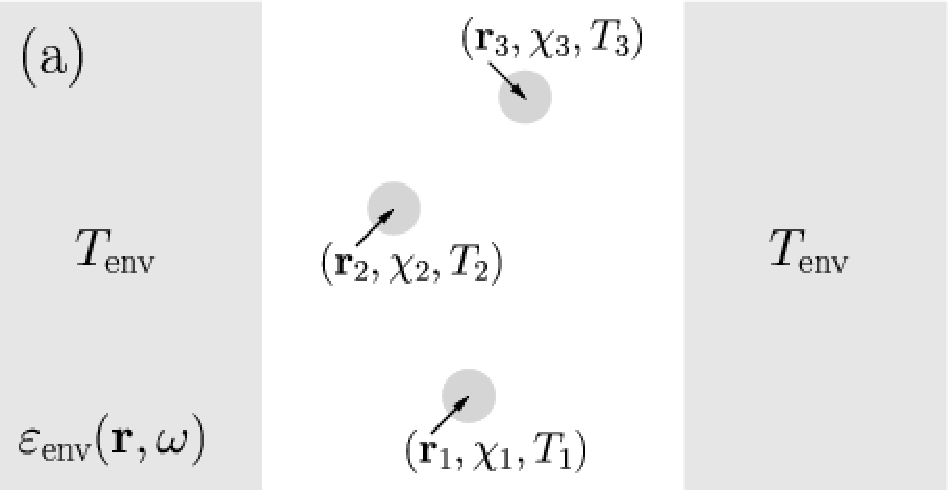
\includegraphics[width=.49\columnwidth]{pics/dipole_pic1a.pdf}
 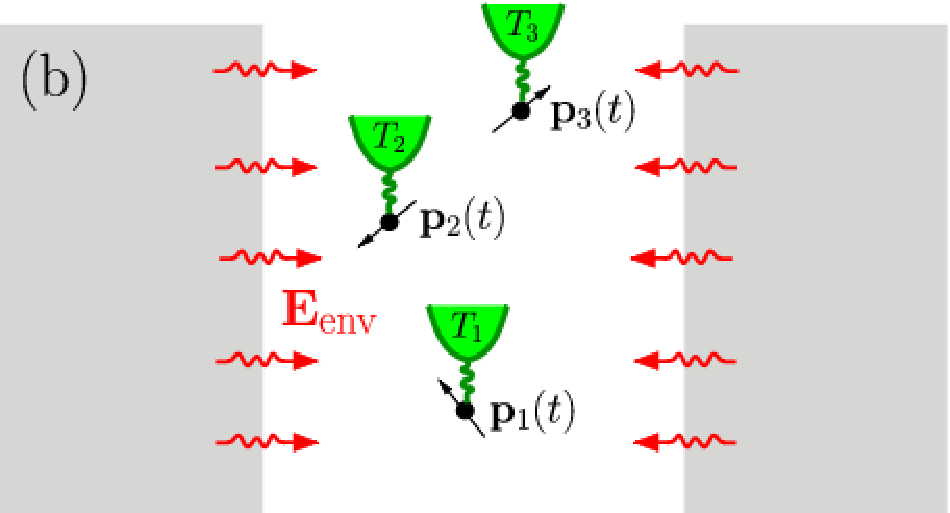
\includegraphics[width=.49\columnwidth]{pics/dipole_pic1b.pdf}
%   \includegraphics[width=.49\columnwidth]{../dipole_resubmission/pic1b}
 \caption{(a) A schematic illustration of the studied electromagnetic energy transfer setup. A collection of dielectric particles with positions $\mathbf{r}_i$, $i\in\{1,\dots,N\}$, electric susceptibilities $\chi_i(\omega)$ and temperatures $T_i$ is located in an inhomogeneous environment, consisting in the shown case of two dielectric (or metallic) bodies forming a cavity. The overall relative permittivity is $\varepsilon(\br,\omega)=\epsenv(\br,\omega)$ outside the particles and $\varepsilon(\br_i,\omega)=1+\chi_i(\omega)$ at the position of each particle coordinate $\br_i$. The two cavity walls, described by the environment dielectric constans, are assumed to act as a source of thermal radiation at temperature $\Tenv$. The polarization field inside each particle $i$ is modeled as an oscillating point dipole moment $\bb{p}_i$ coupled to a local Langevin heat bath at temperature $T_i$ as depicted in (b). The total local field $\bE(\br_i,t)$ driving each dipole moment $\bb{p}_i$ is the sum of the stochastic background field $\bE_{\textrm{env}}(\br_i,t)$ and the fields $\bE_{ij}(t)$ created by each dipole $j$.}%The local bath temperatures $T_i$ correspond to local lattice temperatures, which could either by given fixed temperatures or could be self-consistently determined by the balance of absorption, emission and the in- and outflow of lattice heat. 
\label{fig:gfm_dipole_system}
\end{figure}

This section is devoted to the theory of electromagnetic energy transfer developed in detail in \citepub{dipole}. As discussed in Sec. \ref{sec:intro_emtheory}, we have developed a more microscopic alternative to fluctuational electrodynamics, which is traditionally used to describe electromagnetic energy transfer \cite{joulain05}. Although our final expressions for energy transfer rates are fully equivalent to fluctuational electrodynamics results (see, e.g., Ref. \cite{messina13}), our theory more transparently treats the radiation damping, straightforwardly allows for deriving expressions for heat transfer rates in terms of various different definitions of the local polarizability and allows for coupling the optical degrees of freedom to other degrees of freedom such as acoustic phonons.

We briefly outline our quantum Langevin equation approach to the electromagnetic energy transfer here. More details are found in \citepub{dipole}. The studied system is depicted in Fig. \ref{fig:gfm_dipole_system}. Dielectric particles with positions $\mathbf{r}_i$, $i\in\{1,\dots,N\}$ are located in an inhomogeneous environment characterized by the environment's dielectric constant $\epsenv(\br,\omega)$. For inhomogeneous $\epsenv(\br,\omega)$, the environment acts not only as a source of non-blackbody thermal radiation (at temperature $\Tenv$) but also as a scatterer of the radiation emitted by the particles, thereby modifying the energy transfer rates compared to the free space. The overall relative permittivity is given by $\varepsilon(\br_i,\omega)=1+\chi_i(\omega)$ at the locations of the particles ($\chi_i$ being the electric susceptibility of particle $i$) and $\varepsilon(\br_i,\omega)=\epsenv(\bb{r},\omega)$ elsewhere. The microscopic dipole moments, which represent the fluctuating electric polarization inside each particle, are oupled to (1) local heat baths describing thermal fluctuations and dissipation, (2) to the electromagnetic field arising from other dipoles, and (3) to the thermal field originating from the environment. Following the dipole approximation \cite{novotny}, we assume each particle to be smaller than the optical wavelength so that we can treat the particles as dipoles located at locations $\br_i$, but the theory can be straightforwardly generalized to larger particles as well by dividing the particles into small dipolar volumes as in the traditional discrete dipole method \cite{novotny}. 

%Following the dipole approximation, the internal polarization field of each particle is modeled as a point dipole located at the central coordinate $\br_i$ of the particle $i$ as illustrated in Fig. \ref{fig:sud1}(b). 

\subsubsection{Equation of motion and solution}

The local dynamics of each dipole is modeled by the classical oscillator model accompanied by quantum Langevin dynamics. The equation of motion for the local dipole displacement $\bu_i$, related to the dipole moment through $\bp_i=\bu_i/q$ where $q$ is the charge, reads
 \begin{equation}
 m\ddot\bu_i(t) = -m\omega_i^2 \bu_i(t) +\xi_i(t) -m\gamma_i \dot{\bu}_i(t)  + q \bE_i(t). \label{eq:gfm_eom1}
\end{equation}
The oscillator mass $m$, charge $q$, resonance frequency $\omega_i$ and the friction parameter $\gamma_i$ are absorbed into the definition of the local polarizability in the final expressions. The stochastic force $\xi_i(t)$, which is related to the friction term $m\gamma_i\dot{\bu}_i(t)$ by the standard fluctuation-dissipation relation \eqref{eq:th_xixiom_ohmic_qm}, accounts for thermal fluctuations. 

The steady state solution to the equations of motion can be most easily achieved by moving to frequency domain, in which the equations of motion become
\begin{equation}
 -m\omega^2 \hat\bu_i(\omega) = -m\omega_i^2 \hat\bu_i(\omega) +\hat \xi_i(\omega) +im\gamma_i \omega \hat \bu_i(\omega)  + q \hat \bE_i(\omega). \label{eq:gfm_eom2}
\end{equation}
Here, the Fourier transform of the local electric field $\hat \bE_i$ consists of the environment field $\Eenvhat(\br_i,\omega)$ and the fields $\hat \bE_{ij}(\omega)$ generated by each dipole $j$ [Eq. \eqref{eq:th_Etilde} with spatially localized sources]:
\begin{equation}
 \hat{\bE}_i\pom= \Eenvhat(\br_i,\omega) + \sum_{j=1}^N \hat{\bE}_{ij}\pom. \label{eq:gfm_etot}
\end{equation}
The electric field $\bE_{ij}$ due to dipole moment $\hat{\bb{p}}_j$, responsible for the electromagnetic interaction between the dipoles, is given in frequency domain by [Eq. \eqref{eq:th_Etilde}]
\begin{equation}
 \hat{\bE}_{ij}(\omega) = \omega^2 \mu_0\gem_{ij}(\omega) \hat{\bp}_j (\omega), \label{eq:gfm_ekl}
\end{equation}
where $\gem_{ij}(\omega)\equiv \gem(\br_i,\br_j;\omega)$ is found from Eq. \eqref{eq:intro_gemdef} for given $\epsenv(\br,\omega)$. The stochastic environment field has zero average and satisfies the fluctuation-dissipation relation \cite{novotny}
\begin{alignat}{2}
  q^2 \langle \Eenvhat(\bb{r}_i,\omega) \Eenvhat(\bb{r}_j,\omega')^T \rangle   &=  2\pi \delta(\omega+\omega') \hbar \Gamma^{\textrm{rad}}_{ij}(\omega) \fbbg, \label{eq:gfm_ebgebg1}
\end{alignat}
where the coupling function of the dipoles to the radiation field is
\begin{equation}
 \Gamma_{ij}^{\textrm{rad}}(\omega) = 2 q^2\omega^2\mu_0 \textrm{Im}[\gem_{ij}(\omega)]. \label{eq:gfm_gammarad_def}
\end{equation}

It is important to stress that while the Green's dyadic $\gem$ only accounts for the scattering of the electromagnetic field from the inhomogeneities in the environment, the scattering of the field from the point dipoles is automatically included in the formalism by the coupled dipole equations of motion. The local Green's dyadic $\gem_{ii}(\omega)$, discussed in more detail in \citepub{dipole}, accounts for the Abraham-Lorentz radiation damping, which produces a force term proportional to third time derivative of $\bb{u}$ in the dipole equation of motion \eqref{eq:gfm_eom1}. The fluctuations accompanying the radiation reaction damping are responsible for generating thermal radiation \cite{greffet10}.

The substitution of Eqs. \eqref{eq:gfm_etot} and \eqref{eq:gfm_ekl} to Eq. \eqref{eq:gfm_eom2} gives
\begin{equation}
 -m\omega^2 \hat{\bu}_i \pom =  -m\omega_i^2 \hat \bu_i\pom + \hat{\xi}_i\pom + im\gamma_i \omega \hat{\bu}_i\pom + \Eenvhat(\br_i,\omega) + q^2\omega^2\mu_0 \sum_{j=1}^N \gem_{ij}\pom \hat{\bu}_j\pom. \label{eq:gfm_eom_freq}
\end{equation}
Equation \eqref{eq:gfm_eom_freq} can be rearranged as
\begin{equation}
 - \sum_{j} \bb{A}_{ij} \hat{\bu}_j(\omega) = \hat{\xi}_i(\omega) + q\Eenvhat(\br_i,\omega) \label{eq:gfm_eom_akl}
\end{equation}
by defining an inverse propagator
\begin{equation}
 \bb{A}_{ij} = \left[m(\omega^2-\omega_i^2+i\gamma_i) \right]\delta_{ij}\bb{I}_{3\times 3}+ q^2\omega^2\mu_0 \gem_{ij},
\end{equation}
where $\unitdyadic$ is the $3\times 3$ unit matrix. The solution to Eq. \eqref{eq:gfm_eom_akl} can be written compactly in matrix form as
\begin{equation}
 \hat{\bu}(\omega) = -\bb{G}(\omega) \left[\hat{\xi}(\omega)+q\Eenvhat(\omega) \right], \label{eq:gfm_usol}
\end{equation}
where the dipole displacement Green's function $\bb{G}\pom=\bb{A}\pom^{-1}$ is
\begin{equation}
 \bb{G}(\omega) = \frac{1}{m(\omega^2 \mathbf{I}_{3N\times 3N}-\Omega^2)+q^2\omega^2\mu_0 \textrm{Re}[\gem(\omega)]+i\Gamma^{\textrm{bath}}(\omega)/2+i\Gamma^{\textrm{rad}}(\omega)/2}. \label{eq:gfm_g_expression1}
\end{equation}
Here we adopted a matrix notation where the dipole indices $i\in \{1,\dots,N\}$ and the spatial components $\alpha\in \{1,2,3\}$ are combined into a composite index resulting in matrices and vectors of size $3N\times 3N$ and $3N$, respectively. In the following, we will use an index notation where the subscript $ij$ ($i$) always refers to the $3\times 3$ matrix (3-component vector) corresponding to the notation used before Eq. \eqref{eq:gfm_usol}.

In Eq. \eqref{eq:gfm_usol}, we have additionally defined the block-diagonal resonance frequency matrix as $\Omega=\textrm{diag}(\omega_1\bb{I}_{3\times 3},\omega_2\bb{I}_{3\times 3},\dots,\omega_N\bb{I}_{3\times 3})$ and the block-diagonal bath coupling matrix as $\Gamma^{\textrm{bath}} (\omega) = \textrm{diag}(2m \gamma_1 \omega\bb{I}_{3\times 3},\dots,2m\gamma_N \omega_N \bb{I}_{3\times 3})$.

%In the denominator of Eq. \eqref{eq:g_expression1} and in all matrix-valued expressions appearing below, the scalar terms should be interpreted as being proportional to the unit matrix of size $3N\times3N$.

Equation \eqref{eq:gfm_g_expression1} shows that both the coupling to heat baths and the coupling to the radiation field produce broadening in the Green's function via the coupling functions $\Gamma^{\textrm{bath}}(\omega)$ and $\Gamma^{\textrm{rad}}(\omega)$. This broadening in the Green's function reflects dissipation that, along with the accompanying thermal fluctuations, enables energy transfer between dipoles with different bath temperatures.

\subsubsection{Heat current}

The heat transfer rates between particles could in general be calculated from the electromagnetic Poynting vector, but the calculations can be simplified by energy conservation arguments. A direct calculation shows that the expectation value of the Poynting vector's flux across a surface $\partial V_i$ enclosing a particle $i$, equal to the power of the emitted radiation field, satisfies 
\begin{equation}
 \left\langle \int_{\partial V_i} \bb{S} \cdot d\bb{S} \right\rangle = - \langle Q_i \rangle,
\end{equation}
where the energy current to the bath is given by the bath force multiplied by the dipole moment ''velocity'': $Q_i = (m\gamma \dot{\bu}_i-\xi_i)\cdot \dot{\bu}_i$. Therefore, $\langle Q_i\rangle$ can be interpreted as the locally absorbed power. Direct calculation carried out in \citepub{dipole} shows that 
\begin{alignat}{2}
 \langle Q_i \rangle &= \int_0^{\infty}\frac{d\omega}{2\pi} \hbar\omega \sum_{j} \ca{T}_{ij}(\omega) \left[f_B(\omega,T_j)-f_B(\omega,T_i ) \right] \notag \\
  & \quad + \int_0^{\infty} \frac{d\omega}{2\pi} \hbar \omega \ca{T}_{i,\textrm{rad}}(\omega)\left[ f_B(\omega,\Tenv)-f_B(\omega,T_i)\right].
\end{alignat}
Here the dipole-dipole transmission function is defined as
\begin{equation}
 \ca{T}_{ij}(\omega) = \textrm{Tr} \left[\Gamma_i(\omega) \bb{G}(\omega) \Gamma_j(\omega) \bb{G}(\omega)^{\dagger} \right]
\end{equation}
and the dipole-environment transmission is 
\begin{equation}
 \ca{T}_{i,\textrm{rad}}(\omega) =  \textrm{Tr} \left\{ \Gamma_i(\omega) \left[ \bb{G}(\omega) \Gamma_{\textrm{rad}}(\omega) \bb{G}(\omega)^{\dagger} \right]_{ii} \right\}. \label{eq:th_Tirad}
\end{equation}

\subsubsection{Local polarizabilities}

To calculate the transmission functions, it is useful to express the transmission function in terms of purely optical quantities. This can be achieved by (i) absorbing the microscopic, auxiliary parameters $m$, $q$, $\gamma_i$ to the definitions of the local polarizabilities and (ii) expressing the Green's function in terms of the electromagnetic Green's dyadics. For (i), one must specify the microscopic definition for the polarizability. While there are at least three different definitions available, we use here the Clausius-Mossotti definition 
\begin{equation}
 \langle \hat \bp_i(\omega) \rangle = \varepsilon_0 \alpha_{\textrm{CM}}^i(\omega) \left[\hat \bE_0(\br_i,\omega)+ \left\langle \hat \bE_{\textrm{pol},i} (\omega) \right\rangle \right]
\end{equation}
relating the expectation value of the local dipole moment to the sum of the external field $\bE_0(\br_i,\omega)$ and the polarization field $\bE_{\textrm{pol},i} (\omega)=\hat \bp_i(\omega) /(3\varepsilon_0 \Delta V_i)$ ($\Delta V_i$ is the particle volume). By solving the equation of motion for a single dipole in an external field, one gets 
\begin{equation}
 \alpha_{\textrm{CM}}^i(\omega) = - \frac{q^2}{\varepsilon_0} \frac{1}{m(\omega^2-\omega_i^2+i\gamma_i)-q^2/(3\varepsilon_0\Delta V_i)}\unitdyadic. \label{eq:gfm_alpha_cm_expr}
\end{equation}
One can also start from the microscopic definitions $\varepsilon_i(\omega)=1+\chi_i(\omega)$, $\hat{\bb{P}}(\bb{r}_i,\omega)=\varepsilon_0 \chi_i(\omega) \hat{\bb{E}}(\bb{r}_i,\omega)$ and $\hat{\bb{P}}(\bb{r}_i,\omega)=\hat{\bb{p}}_i(\omega)/\Delta V_i$ to show that
\begin{equation}
 \alpha_{\textrm{CM}}^i(\omega) = 3\Delta V_i \frac{\varepsilon_i(\omega)-1}{\varepsilon_i(\omega)+2} \unitdyadic. \label{eq:gfm_alphacm_epsilon}
\end{equation}
Equations \eqref{eq:gfm_alpha_cm_expr} and \eqref{eq:gfm_alphacm_epsilon} provide the link between the microscopic parameters and the macroscopic dielectric constant $\varepsilon_i(\omega)$ of the particle $i$.

Using Eq. \eqref{eq:gfm_alpha_cm_expr} and straightforward albeit tedious algebraic manipulations, one can write the dipole-dipole energy transmission function as
\begin{equation}
   \ca{T}_{ij}(\omega) = 4 \kw^4 \textrm{Tr} \left[ \textrm{Im}[\alpha^i_{\textrm{CM}}(\omega)] \gemfull_{ij}\pom \textrm{Im}[\alpha^j_{\textrm{CM}}(\omega)] \gemfull_{ji}(\omega)^{\dagger}\right]. \label{eq:tij_final}
\end{equation}
Here the electromagnetic Green's dyadic $\gemfull(\omega)$ expressed in terms of the Clausius-Mossotti polarizabilities of the particles has been defined as 
\begin{alignat}{2}
 \gemfull(\omega) &= \frac{1}{\kw^2} \left[\frac{1}{1-\kw^2 \gem(\omega)\alpha_{\textrm{CM}}(\omega)}\right] \alpha_{\textrm{CM}}(\omega)^{-1} \\
  &\equiv \frac{1}{\kw^2} \alpha_{\textrm{CM}}(\omega)^{-1} + \underbrace{ \left[\frac{1}{1-\kw^2 \gem(\omega)\alpha_{\textrm{CM}}(\omega)} \right] \gem(\omega)}_{\tildegemfull}. \label{eq:gfm_gemmb_cm_app}
\end{alignat}
The first term of Eq. \eqref{eq:gfm_gemmb_cm_app} is local and does not contribute to dipole-dipole energy transfer. The second term of Eq. \eqref{eq:gfm_gemmb_cm_app}, denoted by $\tildegemfull$, is non-local and therefore responsible for dipole-dipole energy transfer. By comparing the expression \eqref{eq:gfm_gemmb_cm_app} to the one obtained from FED \cite{benabdallah11}, one can show that $\tildegemfull$ is readily interpreted as the electromagnetic Green's dyadic that fully incorporates the scattering caused by the dipoles. %In our manuscript, Eq. \eqref{eq:gfm_gemmb_cm_app} arises as a convenient definition that allows us to express the transmission function \eqref{eq:tij_final} in terms of purely optical quantities.

The radiation transmission function \eqref{eq:th_Tirad} can be similarly written in terms of the polarizabilities and the Clausius-Mossotti Green's dyadic as
\begin{alignat}{2}
 \ca{T}_{i,\textrm{rad}}(\omega) 
 &= 4 \kw^6 \sum_{j,k=1}^N \textrm{Tr}\left\{   \textrm{Im}[\alpha^i_{\textrm{CM}}(\omega)] \gemfull_{ij}(\omega) \alpha_{\textrm{CM}}^j(\omega) \textrm{Im}[\gem_{jk}(\omega)] \alpha^k_{\textrm{CM}}(\omega)^* \gemfull_{ki}(\omega)^{\dagger} \right\}. \label{eq:tirad_final}
\end{alignat}
An equation similar to \eqref{eq:tirad_final} was derived very recently before the publication of Publication \cp{dipole} by Messina \textit{et al.} \cite{messina13}.

% The thermal background field $\Eenvhat$ has zero average $\langle \Eenvhat \rangle=0$ and its symmetrized autocorrelation function satisfies the fluctuation-dissipation relation 


% \subsection{Introduction to Green's functions}
% 
% \label{sec:gf_linear}
% Green's function method is based on inverting the ''equation of motion operator'', which we will discuss later. For a general non-homogenous equation of the form
% \begin{equation}
%  \mathcal{L} f = g,
% \end{equation}
% where $\mathcal{L}$ is a linear operator and $g$ is the source function, symbolic solution in terms of the Green's function $\mathcal{G}$ is
% \begin{equation}
%  f = \mathcal{G} g.
% \end{equation}
% The Green's function $\mathcal{G}$ is defined as the inverse of $\mathcal{L}$:
% \begin{equation}
%  \mathcal{L} \mathcal{G} = I,
% \end{equation}
% where $I$ is the identity operator. Since $\mathcal{L}$ is linear, solution for 
% \begin{equation}
%  \mathcal{L} f = g_1 + g_2
% \end{equation}
% is the sum of solutions
% \begin{equation}
%  f = \mathcal{G}g_1 + \mathcal{G} g_2.
% \end{equation}
% Calculating $\mathcal{G}$ for a given $\mathcal{L}$ determines, therefore, the solution for any source function $g$. 
% 
% 
% 
% \subsection{Quantum mechanical Green's functions}
% 
% For completeness, we also briefly discuss the Green's functions that appear in the quantum-mechanical many-body problem. These functions are directly defined as statistical averages of different correlation functions and, at first sight, bear no resemblance to the Green's function discussed in Sec. \ref{sec:gf_linear}. The most used two-particle Green's functions are \cite{wang08}
%  \begin{alignat}{2}
%    G^R(t,t') &= -i\theta(t-t') \langle [\bb{u}(t), \bb{u}(t')^T] \rangle \\
%    G^A(t,t') &= i\theta(t'-t) \langle [\bb{u}(t), \bb{u}(t')^T] \rangle\\
%    G^>(t,t') &= -i\langle \bb{u}(t) \bb{u}(t')^T \rangle\\
%    G^<(t,t') &= -i\langle \bb{u}(t') \bb{u}(t)^T \rangle^T	 \\
%    G^t(t,t') &= \theta(t-t') G^>(t,t') + \theta(t'-t) G^<(t,t') \\
%    G^{\bar t}(t,t') &=\theta(t'-t) G^>(t,t') + \theta(t-t') G^<(t,t')  ,
%  \end{alignat}
% which are called the retarded, advanced, greater, lesser, time-ordered and anti-time-ordered Green's functions, respectively. The operators appearing inside the expectation values are written in Heisenberg picture. Out of the six Green's functions, only three are linearly independent and, in steady-state, the number of independent functions is reduced to two. In equilibrium, one of the Green's functions determines the others, and typically $G^R$ is considered. Note that $G^R$ satisfies
% \begin{alignat}{2}
%  \partial_t G^R(t,t')  &= -i \delta(t-t')  \langle [\bb{u}(t), \bb{u}(t')^T] \rangle -i \theta(t-t') \langle [\dot{\bb{u}}(t),\bb{u}(t')^T ] \rangle \\
%   &= -i \theta(t-t') \langle [\bb{p}(t),\bb{u}(t') ]^T \rangle
% \end{alignat}
% and
% \begin{alignat}{2}
%  \partial_t^2 G^R(t,t') &= - i \delta(t-t') \langle [\bb{p}(t),\bb{u}(t') ]^T \rangle - i \theta(t-t') \langle [\dot{\bb{p}}(t),\bb{u}(t')^T] \rangle \\
%   &= - \delta(t-t')\bb{I}  - i \theta(t-t') \langle [\dot{\bb{p}}(t),\bb{u}(t')^T] \rangle .
% \end{alignat}
% For a quadratic Hamiltonian 
% \begin{equation}
%  \mathcal{H} = \frac{\bb{p}^2}{2} + \frac{1}{2} \bb{u}^T \bb{K} \bb{u},
% \end{equation}
% the Heisenberg equation of motion for $\bb{p}(t)$ is 
% \begin{equation}
%  \dot{\bb{p}}(t) = - \bb{K} \bb{u}(t),
%  \label{eq:dotpt}
% \end{equation}
% so 
% \begin{equation}
%  \partial_t^2 G^R_{ij} (t,t') = - \delta(t-t') \delta_{ij} - K_{ik} G^R_{kj}(t,t').
% \end{equation}
% Fourier transformation then gives the familiar Green's function
% \begin{equation}
%  G^R(\omega) = [(\omega+i\eta)^2-\bb{K}]^{-1}
% \end{equation}
% from the last section. This short calculation justifies the name Green's function. Note that for an interacting system, Eq. \eqref{eq:dotpt} would not be valid and the hiearchy of equations of motion would not close.
% 
% The usefulness of Green's functions in the statistical mechanics of quantum-mechanical systems lies in the facts that (1) they can be used to calculate all thermodynamic observables \cite{negele}, and (2) they allow an easy and intuitive perturbative expansion that can be represented as Feynman diagrams \cite{negele,fetter2}. At zero and non-zero temperature, the diagrammatic expansion in terms of the interaction parameter is carried out for the time-ordered Green's function and the Matsubara Green's function, respectively. Methods such as functional renormalization group \cite{metzner12,saaskilahti11} can be applied to sum a subset of diagrams up to an infinite order in a controlled manner.
% 
% In the context of non-equilibrium transport problem, Meir and Wingreen showed that the electronic current through an \textit{interacting} system can be written in terms of $A(\omega)$, the spectral function of the system. Corresponding formula for phonon transport through an anharmonic system was derived by Wang \cite{wang06} and Mingo \cite{mingo06}, and the formula reads for, say, the current flowing to the left lead
% \begin{equation}
%  I = \int \frac{d\omega}{2\pi} \omega \textrm{Tr}\left[G^R(\omega) \Sigma^<(\omega) + G^<(\omega) \Sigma^A(\omega) \right],
% \end{equation}
% where $\Sigma^<$ and $\Sigma^A$ are the lesser and advanced self-energies of the left lead. To calculate the Green's functions and self-energies perturbatively, the perturbation expansion is done for the more general Keldysh Green's function
% \begin{equation}
%  G (\tau,\tau') = -i \langle \mathcal{T}_{\tau} u(\tau) u(\tau') \rangle.
% \end{equation}
% Time variable $\tau$ lies on the Keldysh contour, which runs from $-\infty$ to $\infty$ slightly above the real axis and back to $-\infty$ slightly below the real axis \cite{jauho}.



%\begin{itemize}
% \item Definition of polarizability, optical theorem
% \item Coupling of optical and acoustic degrees of freedom
%\end{itemize}


\iffalse
\begin{equation}
 \left\langle \tilde{j}^{\alpha}(\br,\omega)\tilde{j}^{\beta}(\br',\omega') \right\rangle = 2\pi \delta(\omega+\omega') \times 2\omega \varepsilon_0 \textrm{Im}[\varepsilon(\br,\br';\omega)] \hbar \omega \left[f_B(\omega,T)+\frac{1}{2} \right]
\end{equation}
\fi
%\begin{itemize}
% \item Maxwell equations
% \item Fluctuational electrodynamics
% \item Electromagnetic Green's function
%\end{itemize}
% Loomis and Maris 94: We present a macroscopic, phenomenological theory for the heat flow between two material half-spaces of differing temperatures whose surfaces are separated by a gap of width l. Our calculation parallels Liftshitz's calculation of the van der Waals force between two dielectric slabs. For l sufficiently small, the heat flow is enhanced by a contribution from evanescent waves, and in the limit of a very small gap varies as l^{-2}.




\iffalse
Usually, the bath self-energy $\Sigma(\omega)$ is given to specify the coupling with the bath. Therefore, it is useful to derive an expression relating the bath self-energy to $M(t)$. This process is complicated by the fact that because $M(t)$ does not vanish at negative infinity, one cannot use the Fourier transform of $M(t)$ in the process. However, because only the values of $M(t)$ for $t>0$ play a role in Eq. \eqref{}, one can introduce a step-function in the integral and substitute the convenient definition $M^e(t)=\Theta(t)M(t)+\Theta(-t)M(-t)$:
\begin{equation}
 m\ddot{u}(t) =  F[u(t)] - \int_{-\infty}^{\infty}dt'\Theta(t') M^e(t')\dot{u}(t-t') + \xi(t).
\end{equation}
One can then easily show that the Fourier transform of $M^e(t)$ is related to the bath self-energy $\Sigma(\omega)$ through the coupling function $\Gamma(\omega)=-2\textrm{Im}[\Sigma(\omega)]$:
\begin{equation}
 \hat M^e(\omega) = \frac{\Gamma(\omega)}{\omega}. \label{eq:th_langevin_Mt}
\end{equation}
In cases where the exact spectral properties of the bath do not matter, the simplest choice for the bath self-energy is
\begin{equation}
 \Sigma(\omega) = -i\gamma \omega \Theta(\omega_c-|\omega|),
\end{equation}
where $\omega_c$ is the cut-off frequency for the bath modes. Equation \eqref{eq:th_langevin_Me} then gives
\begin{equation}
 \hat M^e(\omega) = 2\gamma \Theta(\omega_c-|\omega|), 
\end{equation}
so the friction kernel $M^e(t)$ is 
\begin{equation}
 M^e(t) = 2 \gamma \delta_{\omega_c}(t),
\end{equation}
where 
\begin{equation}
 \delta_{\omega_c} (t) = \frac{1}{\pi} \frac{\sin \omega_c t}{t}. \label{eq:th_langevin_deltat}
\end{equation}
For $\omega_c\to \infty$, Eq. \eqref{eq:th_langevin_deltat} tends to the Dirac Delta function and the friction term in the generalized Langevin equation reduces to the classic Langevin equation 
\begin{equation}
  m\ddot{u} = {F}[{u}(t)] -m \gamma \dot{{u}} + \xi(t). 
\end{equation}
\fi
\iffalse

\subsection{Background}
In his seminal work on the theory of Brownian motion, Paul Langevin added stochastic force terms in the equation of motion to model the essentially random collisions of a particle with the molecules of the surrounding fluid. The additional force consists of two terms, the deterministic damping force proportional to the friction coefficient $\gamma$ and the stochastic force $\xi$:
\begin{equation}
 m \ddot{x} = {F}[{x}(t)] -m \gamma \dot{{x}} + \xi(t). \label{eq:langevin_eq}
\end{equation}
Here ${x}(t)$ is the particle position, $m$ the mass and ${F}[{x}(t)]$ is the force due to particles other than the solvent. For simplicity, we have written the one-dimensional form of the equation. In Langevin theory, the collisions with the solvent (represented by the stochastic force $\xi$) are assumed to average to zero force ($\langle \xi \rangle=0$) and to be temporally uncorrelated: $\langle \xi(t) \xi(t')^T\rangle \propto \delta(t-t')$. To calculate the constant of proportionality in the variance, one can calculate the expectation value of $\langle v^2\rangle$ for $t \to \infty$ to show that the classical equipartition $ m \langle \bb{v}^2 \rangle = k_BT$ only holds if the stochastic force and friction force are related by the relation
\begin{equation}
 \langle \xi(t) \xi(t')\rangle=2\gamma T \delta(t-t'). \label{eq:corr_ohmic} %\mathbf{I}_{3\times 3}
\end{equation}
This is the fluctuation-dissipation relation connecting the magnitude of fluctuations $\xi$ to the dissipation constant $\gamma$. The damping term of Eq. \eqref{eq:langevin_eq} is often referred to as Ohmic damping due to its correspondence with an Ohmic resistor in circuit theory \cite{weiss}.

In this example, the molecules of the solvent act as a thermal reservoir at temperature $T$. For any given initial velocity of the particle, the particle will drift toward thermal equilibrium with the reservoir and eventually achieve it. Building on this idea, Langevin forces are traditionally used in simulations to thermostat the system to a given temperature \cite{}. This allows one to either (i) simulate canonical ensemble at given temperature, (ii) push the system into thermal non-equilibrium by coupling atoms to Langevin thermostats at different temperatures, or (iii) to simulate dissipative and fluctuative processes driving the system to local equilibrium by Langevin thermostats at position-dependent temperatures.
\fi
\iffalse
\section{Langevin bath in simulations}

Langevin bath is typically used for three different tasks. In the first case, Langevin bath is used to simulate canonical ensemble (thermal equilibrium) by coupling all atoms to a bath at single temperaure $T$. In this case, the coupling constant $\gamma$ to the baths should typically be chosen small enough so that the coupling does not disturb the natural vibrational dynamics in the system. If the coupling is too small, however, the energy exchange with the bath is so slow that very long simulation runs are required to properly sample the available phase space.

In the second case, multiple baths at different temperatures are used to push the system into non-equilibrium. In this case, the baths act as heat sources and sinks, and the coupling constant $\gamma$ effectively determines the contact resistance with the reservoirs. While large $\gamma$ generally decreases the contact resistance to the reservoirs, it also increases the acoustic mismatch between thermalized and unthermalized atoms. Therefore, it should be carefully checked that the obtained results (such as thermal resistance) are not sensitive to the exact value of $\gamma$.

Finally, coupling to the Langevin bath can describe \textit{internal} processes driving the system into (local) thermal equilibrium. For example, the complicated phonon-phonon interactions giving rise to phonon creation and annihilation can be described in an effective manner by the fluctuating and dissipative Langevin forces, respectively. The resulting linearization of the equations of motion allows for solving the equations of motion directly in terms of the Green's function. To ensure current conservation, it is necessary to determine the bath temperatures self-consistently so that phonon creation and annihilation are balanced. This is the self-consistent heat bath model.
\fi

\iffalse
\subsection{General Langevin equation}

The original Langevin equation with the classical fluctuation-dissipation relation is typically used in molecular dynamics simulations due to its simplicity. In cases when the spectral properties of the coupling to the bath matter (for example to minimize the contact resistance between the bath and the system) or if quantum statistics must be accounted for, one must turn to the general Langevin theory \cite{weiss}.

In general Langevin theory, the reservoir is modeled as a collection of harmonic oscillators. The bath degrees of freedom are ''integrated out'' so that their interaction with the system under study is described effectively by the Langevin forces. In general, the friction and force then have temporal correlations and the Ohmic damping of Eq. \eqref{eq:langevin_eq} and Markovian force [Eq. \eqref{eq:corr_ohmic}] are replaced by more complicated expressions \cite{weiss}. The general Langevin equation reads \cite{dhar06}
\begin{equation}
 m\ddot{u}(t) =  F[u(t)] - \int_{0}^{\infty}dt' \Sigma(t') {u}(t-t') + \xi(t),
\end{equation}
where the auto-correlation function of the random force $\xi$ is related to the damping self-energy through the fluctuation-dissipation relation
\begin{equation}
 \langle \xi(t)\xi(t') \rangle = \int_{-\infty}^{\infty} \frac{d\omega}{2\pi} e^{-i\omega(t-t')} \hbar \Gamma(\omega) [f_B(\omega,T)+1].
\end{equation}
By Fourier transforming with respect to $t$ and $t'$ separately, Eq. (XXX) can be written in the form useful for calculations:
\begin{equation}
  \langle \xi(\omega)\xi(\omega') \rangle = 2\pi\hbar\delta(\omega+\omega') \Gamma(\omega) \left[f_B(\omega,T)+1 \right].
\end{equation}
Here $\Gamma(\omega)=-2\textrm{Im}[\Sigma(\omega)]$.

Typically, the integral term in the Langevin equation is written in terms of the velocity to identify it as a frictional force. To achieve this, we integrate partially in Eq. \eqref{}:
\begin{equation}
 m\ddot{u}(t) =  F[u(t)] - \int_{0}^{\infty}dt' M(t')\dot{u}(t-t') + \xi(t)
\end{equation}
The boundary terms in the integral are assumed to vanish  because we (i) define the integral function $M(t)=-\int_t^{\infty} dt' \Sigma(t')$ of $\Sigma(t)$ so that $M(t\to \infty)=0$ and (ii) the term proportional to $M(0)u(t)$ can be absorbed to the external force $F[u(t)]$ or eliminated by re-defining the displacements \cite{weiss}. 

Usually, the bath self-energy $\Sigma(\omega)$ is given to specify the coupling with the bath. Therefore, it is useful to derive an expression relating the bath self-energy to $M(t)$. This process is complicated by the fact that because $M(t)$ does not vanish at negative infinity, one cannot use the Fourier transform of $M(t)$ in the process. However, because only the values of $M(t)$ for $t>0$ play a role in Eq. \eqref{}, one can introduce a step-function in the integral and substitute the convenient definition $M^e(t)=\Theta(t)M(t)+\Theta(-t)M(-t)$:
\begin{equation}
 m\ddot{u}(t) =  F[u(t)] - \int_{-\infty}^{\infty}dt'\Theta(t') M^e(t')\dot{u}(t-t') + \xi(t).
\end{equation}
One can then easily show that the Fourier transform of $M^e(t)$ is related to the bath self-energy $\Sigma(\omega)$ through the coupling function $\Gamma(\omega)=-2\textrm{Im}[\Sigma(\omega)]$:
\begin{equation}
 \hat M^e(\omega) = \frac{\Gamma(\omega)}{\omega}.
\end{equation}
%The fluctuation-dissipation relation then becomes
%\begin{equation}
% \langle \xi(\omega)\xi(\omega') \rangle = 2\pi\hbar\delta(\omega+\omega') \omega M^e(\omega) \left[f_B(\omega,T)+1 \right].
%\end{equation}


\subsection{Ohmic damping}
In cases where the exact spectral properties of the bath do not matter, the simplest choice for the bath self-energy is
\begin{equation}
 \Sigma(\omega) = -i\gamma \omega \Theta(\omega_c-|\omega|),
\end{equation}
where $\omega_c$ is the cut-off frequency for the bath modes. Equation (XXX) then gives
\begin{equation}
 \hat M^e(\omega) = 2\gamma \Theta(\omega_c-|\omega|), 
\end{equation}
so the friction kernel $M^e(t)$ is 
\begin{equation}
 M^e(t) = 2 \gamma \delta_{\omega_c}(t),
\end{equation}
where 
\begin{equation}
 \delta_{\omega_c} (t) = \frac{1}{\pi} \frac{\sin \omega_c t}{t}.
\end{equation}
For $\omega_c\to \infty$, Eq. (XXX) tends to the Dirac Delta function and the friction term in the generalized Langevin equation reduces to the Ohmic damping in the classic Langevin equation (XXX).
\fi
%\section{Langevin theory}

